\documentclass[twocolumn]{emulateapj}
\usepackage{subfigure}
\usepackage{bm}
\usepackage{amsmath, amssymb}
\usepackage{times}
\usepackage[usenames]{xcolor}
\definecolor{mpl_red}{HTML}{D62728}
\usepackage[backref, breaklinks, plainpages=false, colorlinks=true, anchorcolor=blue!50!black, citecolor=blue!50!black, linkcolor=blue!50!black, urlcolor=mpl_red, bookmarks=false]{hyperref}
\citestyle{apj}
\usepackage[strict]{changepage}

\usepackage{natbib}


\begin{document}

% Add bracket to sectioning in the bibliography.
\renewcommand*{\backref}[1]{[#1]}

% Definition of shortcut commands.
\newcommand{\Bansal}{Karishma~Bansal}
\newcommand{\Pearlman}{\href{https:/orcid.org/0000-0002-8912-0732}{\textcolor{blue!50!black}{Aaron~B.~Pearlman}}}
\newcommand{\Majid}{\href{https:/orcid.org/0000-0002-4694-4221}{\textcolor{blue!50!black}{Walid~A.~Majid}}}
\newcommand{\Prince}{\href{https:/orcid.org/0000-0002-8850-3627}{\textcolor{blue!50!black}{Thomas~A.~Prince}}}
\newcommand{\Younes}{George~Younes}
\newcommand{\Hu}{Chin-Ping Hu}
\newcommand{\Enoto}{Teruaki~Enoto}
\newcommand{\Wharton}{Robert~S.~Wharton}
\newcommand{\Kocz}{Jonathan~Kocz}
\newcommand{\Horiuchi}{Shinji~Horiuchi}

\newcommand{\JPL}{Jet Propulsion Laboratory, California Institute of Technology, Pasadena, CA 91109, USA; \textcolor{blue}{karishma.bansal@jpl.nasa.gov}}
\newcommand{\CaltechPhysics}{Division of Physics, Mathematics, and Astronomy, California Institute of Technology, Pasadena, CA 91125, USA}
\newcommand{\GWU}{Department of Physics, The George Washington University, Washington, DC 20052, USA}
\newcommand{\APSIS}{Astronomy, Physics and Statistics Institute of Sciences (APSIS), The George Washington University, Washington, DC 20052, USA}
\newcommand{\RIKEN}{Extreme Natural Phenomena RIKEN Hakubi Research Team, RIKEN Cluster for Pioneering Research, 2-1 Hirosawa, Wako, Saitama 351-0198, Japan}
\newcommand{\Taiwan}{Department of Physics, National Changhua University of Education, Changhua 500, Taiwan}
\newcommand{\berkeley}{Department of Astronomy, University of California, Berkeley, CA 94720, USA}
\newcommand{\CSIRO}{CSIRO Astronomy and Space Science, Canberra Deep Space Communications Complex, P.O. Box 1035, Tuggeranong, ACT 2901, Australia}
\newcommand{\NDSEG}{$^{\text{9}}$~NDSEG Research Fellow.}
\newcommand{\NSF}{$^{\text{10}}$~NSF Graduate Research Fellow.}

%%%%%%%%%%%%%%%%%%%%%%%%%%%%%%%%%%%%%%%%%%%%%%%%%%%%%%%%%

\journalinfo{{\sc Submitted to The Astrophysical Journal Letters}}
\submitted{Submitted to The Astrophysical Journal}

\shorttitle{RADIO AND X-RAY OBSERVATION OF J1818}
\shortauthors{BANSAL ET AL.}

\title{Simultaneous Radio and X-ray observations of a Radio Magnetar: Swift J1818.0$-$1607}

\author{\Bansal\altaffilmark{1}, \Pearlman\altaffilmark{2,9,10}, \Majid\altaffilmark{1,2}, \Prince\altaffilmark{2,1}, \Younes\altaffilmark{3,4}, \Hu\altaffilmark{5,6},  \Enoto\altaffilmark{5},\Wharton\altaffilmark{1}, \Kocz\altaffilmark{2,7}, and~ \Horiuchi\altaffilmark{8}}

\address{
$^{\text{1}}$~\JPL \\
$^{\text{2}}$~\CaltechPhysics \\
$^{\text{3}}$~\GWU \\
$^{\text{4}}$~\APSIS \\
$^{\text{5}}$~\RIKEN \\
$^{\text{6}}$~\Taiwan\\
$^{\text{7}}$~\berkeley\\
$^{\text{8}}$~\CSIRO}
\thanks{\NDSEG}
\thanks{\NSF}

 \begin{abstract}
Swift J1818.0$-$1607 is a recently discovered magnetar with a short spin period of 1.36 s and a magnetic field of $\sim 10^{14}$ Gauss. With an average estimated age of about 500 years, it is one of the youngest known isolated neutron stars with properties blurring the lines between high-B rotation-powered pulsars and magnetars. We have observed this source during multiple epochs, over a span of about six months, at high radio frequencies ($S$, $X$, and $Ka$ bands) using the NASA Deep Space Network. In addition, we have observed it at two epochs in X-ray using the Neutron Star Interior Composition Explorer (NICER) telescope. We discover an anti-alignment (0.40 phase cycles) in the pulse profiles of its simultaneous radio and X-ray observations. We discuss different models to explain this large phase offset, which is likely due to the X-ray emission originating at the base of the hotspots and radio from the closed field lines. Moreover, we report its radio properties, such as a variation in the radio flux densities on the time scales of hours to months; a change from steep ($\alpha < -2.2$) to flat spectra ($\alpha = +0.3$) in about three weeks, followed by a spectral turnover at higher frequencies in a span of about three months, and the varying number of radio pulse profile components.  

%we discuss different models to explain the phase anti-alignment  in the pulse profiles of its simultaneous radio and X-ray observations. There is a marginal change in it over the two epochs. which are anti-aligned in phase.  suggesting a discrepancy in the underlying emission mechanisms and possibly due to the difference in the location of their origin.
\end{abstract}

\section{Introduction}
%Neutron stars exist in various flavors, including radio millisecond pulsars, isolated radio pulsars, magnetars or as X-ray binary systems. Their magnetic field strength ranges from $10^{8}$ Gauss in millisecond pulsars to $10^{15}$ Gauss in magnetars. The origin of the magnetic field in neuton star is due to the conservation of magnetic flux in the core collapse of a supernova. It is likely amplified in the case of magnetars due to the anisotropic super-fluid inside the neutron star core \citep{peng2016}. Nearly $>2700$ in the ATNF catalog known pulsars are classified as radio powered pulsars which have period on the range from 1.4 ms to 25 s. %\abp{[There are 2719 radio pulsars in the ATNF catalog. There are actually more than this, based on compiling PSRs from other catalogs that don't appear in the ATNF. I think $>$\,2700 radio pulsars \textbf{in the ATNF catalog} is more accurate. There's also a LOFAR-discovered PSR with a $\sim$25\,s period.]} \abp{[This sentence is a little confusing to me. Which fields are enormous - magnetars, MSPs, or both? You might want rework this sentence also since the origin of the fields in NSs is very complicated (not fully understood). The thinking used to be (maybe still is?) that they originate from a seed field in a dynamo shortly after core-collapse supernovae. The fields are all stronger toward the core, in fact, by a few orders of magnitude or so.]}

Magnetars are neutron stars with large spin periods of P = $2-12$ s and extreme magnetic fields (B$> 10^{14}$ G). So far about 30 magnetars have been detected, and most of them were detected in the X-ray from either the emission of energetic bursts or pulsed emission \citep{kaspi2017}. Both of these emissions can be explained by the magnetar model \citep{duncan1992,paczynski92}. The persistent X-ray emission is expected from hotspots above the magnetic poles whereas, the X-ray bursts probably originate due to the large magnetic stress or the split and recombination of magnetic field lines. 
The luminosity of magnetar's persistent X-ray emission ranges between $10^{33}$ and $10^{35}$ erg s$^{-1}$ \citep{thompson2002,lyutikob2003}. Magnetars are highly variable, undergoing outburst episodes in conjunction with energetic short bursts, and during that time the number of photons increases. Based on their properties, these bursts can be divided into two main classes: giant flares \citep{palmer2005} and short X-ray bursts. Giant flares have an initial spike lasting a few milliseconds, followed by a minute-long exponentially decaying tail. These giant flares have a peak luminosity of $10^{44} - 10^{47}$ erg s$^{-1}$ and are very rare with a rough occurrence of once per decade. Short X-ray bursts are the most common bursts and have a duration of about a few milliseconds to seconds, and a peak luminosity in the range of $10^{36} - 10^{43}$ erg s$^{-1}$.%ADD REFERENCES 
 
 
Magnetars were believed to be radio-quiet until the first radio-emitting magnetar XTE J1810--197 was discovered \citep{camilo2006}. In addition, four other radio magnetars, namely: PSR J1745--2900 \citep{eatough2013}, PSR J1622--4950 \citep{levin2010}, 1E 1547.0--5408 \citep{camilo20071e}, and SGR 1935+2154 \citep{zhu2020}, along with a transitional magnetar PSR J1119--6127 \citep{Majid+2017, pearlman2019b}, have been discovered. Their properties, such as the flux density, change on the timescale of seconds to months, and the number of components in their profile may also change. Most of these magnetars shut down their emission for some period and typically re-emitting a burst in X-ray. 
%\textbf{Recently, periodic radio emission has been detected from SGR 1935+21 so far}. 

Swift J1818.0$-$1607 (hereafter, J1818) is the sixth magnetar to exhibit radio emission. It was discovered recently on March 12, 2020, when the Burst Alert Telescope was triggered by a soft gamma-ray-burst (GCN 28055). Subsequent follow up observations in X-ray \citep{esposito20} and radio \citep{Champion_2020} have found a spin period of $1.36$ s and $\dot{P} = 8.160 \pm 2 \times 10^{-11}$ s s$^{-1}$, suggesting a magnetic field of $3.4 \times 10^{14}$ G. Compared to typical magnetars, J1818 has one of the smallest spin periods, which is comparable to radio powered pulsars. Its profile has been found to be $80-100 \%$ linearly polarized across a wide observing band \citep{lower2020}. With an average characteristic age of $500$ yrs \citep{Champion_2020}, it is the youngest known magnetars so far. %Hence, this young age magnetar may also serve as a bridge between radio pulsars to magnetars. 
%The recent discovery of FRB 200428 from SGR 1935+21 \wam{ref bochenek20, chime20} suggest that origin of some Fast Radio Bursts (FRBs) is magnetars. This suggests that this source is a bridge between magnetars and FRBs. %radio pulsars have relatively shorter pulse periods, there needs to be a mechanism which explains how magnetars from large period end up spinning faster or something else? I wonder if all these sources pulsar s, magnetars, RRATs, FRBs are just different way to looking at a neutron star. Just like AGNs come in a range of sources - and it is all a matter of orientation.  The X-ray pulse profile exhibits a single broad peak \citep{}. What can we say about a source from its x-ray data?Is it accreting? -  Change in frequency derivative at X-ray frequencies. Spindown luminosity -- $4\pi^2 I Pdot/P^3$ 

In this article, we compare the simultaneous radio and X-ray observations of J1818 using the NASA Deep Space Network (DSN; \citealt{pearlman2019b}) and the Neutron Star Interior Composition Explorer (NICER) telescope, respectively. We also study how the spectral properties of J1818's radio emission evolve over time. Based on these results, we draw comparisons of J1818 with other magnetars and typical radio pulsars. In Section 2.1 and 2.2, we describe our radio observations over six epochs and X-ray observations at two epochs. Then we discuss radio profile analysis in Section 3.1; radio spectral index in Section 3.2; our burst search in the X-ray data in Section 3.3; and X-ray profile in Section 3.4. We discuss these results and our implementations in Section 4 and summarize them in Section 5.

\section{Observations}
%X-ray observations were carried out using the NICER telescope, whereas radio observations using the DSN, as detailed below. 
\subsection{Radio Observations}

We carried out radio observations of J1818 during six epochs using different DSN radio telescopes (Table 1). The first two epochs (2020 March 15 and 2020 March 16) were carried out using DSS-35 and DSS-36, two 34\,m diameter radio telescopes in Canberra, Australia. Subsequent observations on 2020 March 26, 2020, April 08, and 2020 July 15 (Epoch 3, 4, and 5) were carried out using DSS-63, a 70\,m diameter radio telescope in Robledo, Spain. The most recent observation on 2020 August 10 (Epoch 6) was made using the DSS-35.

These observations were carried out in simultaneous dual frequency bands, in dual circular polarization mode, with center frequencies either at 2.2/8.4 GHz ($S$-band/$X$-band) or 8.4/32 GHz ($X$-band / $Ka$-band) as noted in Table~1. The usable bandwidth was roughly 110 MHz at $S$-band, 350 MHz at $X$-band, and 350 MHz at $Ka$-band. Data from both polarization channels in each frequency band were recorded in filterbank format containing channelized power spectral densities with the pulsar machines at each DSN complex, as described previously (e.g., ~\citealt{pearlman2018, pearlman2019b, Majid+2020, pearlman2020bright}). The time and frequency resolution for Epochs 1, 2, and 6 were roughly 512\,$\mu$s, and 1\, MHz respectively. For epochs 3--5, the time and frequency resolution were roughly 2.2\, ms and 0.46\, MHz respectively. Additional information for each epoch, including the date and the starting time of each observing session, and its duration, are provided in Table~1.

% using the pulsar backend in filterbank search mode. The Epoch 1 and Epoch 6 were observed in X and Ka bands centered at 8.3 and  31.9 GHz with a bandwidth of $\sim 352$ and $\sim 353$ MHz, respectively. Epoch 2 was observed at S and X bands centered at 2.3 and 8.4 GHz with a bandwidth of $\sim 118$ and $\sim 432$ MHz. Epoch 3--5 were observed at S and X bands centered at 2.3  and 8.4 GHz with a bandwidth of $\sim 110$ and $\sim 396$ MHz. However, note that these observations differ from one another in their observation duration. More details related to these observations can be found in Table 1. 

%These epochs were observed at center frequencies of 2.3 GHz (S-band) and 8.4 GHz (X-band). The DSN observations were performed simultaneously at the two frequency bands on 2020 March 26, starting at 08:30:00 UTC, for 7440 s (Epoch 1) and on 2020 April 8, starting at 07:37:54 UTC, for 6840 s (Epoch 2). Dual circular polarization data were recorded with bandwidths of $\sim110$ MHz at S-band and $\sim$396 MHz at X-band using the pulsar backend in filterbank search mode with a frequency and time resolution of 0.46 MHz and 2.2 ms, respectively.

The data processing procedures follow similar steps to those presented in previous studies of pulsars and magnetars with the DSN ~(e.g.,~\citealt{Majid+2017, pearlman2018, pearlman2019b, pearlman2020bright}). Each data set was first corrected for bandpass slope across the frequency band. Subsequently, to remove low-frequency temporal variability, the moving average from each data value was subtracted using a 10 s window around each time sample. This was followed by the identification and masking of bad channels corrupted by radio frequency interference (RFI). The two polarization channels for each frequency band were then summed to form a total intensity time series. Each data set was then dedispersed at the nominal DM value of 706\,pc\,cm$^{\text{--3}}$ \citep{lower2020} and barycentered to the R.A. (J2000)$ =18^{h}18^{m}0.12^{s}$ and Decl. (J2000)$= -16^{\circ} 07{^\prime}52.80^{\prime\prime}$. %\abp{[Stokes I is formed before dedispersion; this is done after rfi masking. The order is a little off here. It should be 1. bandpass correction, 2. baseline removal, 3. rfi mitigation, 4. stokes I combination]} 
                                                                      

\begin{deluxetable*}{ccccccc}
    \tablenum{1}
    \tabletypesize{\small}
    \tablecolumns{7}
    \tablewidth{0pt}
	\footnotesize
	\tablecaption{Radio Observations of Swift J1818.0-1607 with the DSN}
    \tablehead{
        \colhead{Epoch} &
        \colhead{Telescope} &
        \colhead{Frequency Bands} &
	    \colhead{Date$^{\mathrm{a}}$} &
        \colhead{Time$^{\mathrm{a}}$} &
        \colhead{Date$^{\mathrm{b}}$} &
        \colhead{Duration} \\
        \colhead{} &
        \colhead{} &
        \colhead{} &
		\colhead{} &
        \colhead{(hh:mm:ss)} &
        \colhead{(MJD)} &
		\colhead{(hr)}
        }
        \startdata
	1 & DSS-35 & X/Ka&2020 Mar 15 & 21:14:60 & 58923.88541 & 0.7 \\
	2 & DSS-36 & S/X & 2020 Mar 16 & 23:00:01 & 58924.95833 & 1.9 \\
	3 & DSS-63 & S/X & 2020 Mar 26 & 08:29:60 & 58934.35417 & 2.1 \\
	4 & DSS-63 & S/X & 2020 Apr 08 & 07:37:54 &  58947.31799 & 1.9 \\
	5 & DSS-63 & S/X & 2020 Jul 15 & 19:46:38 &  59045.82405 & 2.1 \\
	6 & DSS-35 & X/Ka & 2020 Aug 10  & 10:30:00 & 59071.43750 & 1.6 \\
        \enddata
        \tablecomments{At every epoch, datasets in the stated frequencies bands were acquired simultaneously.\\
                $^{\mathrm{a}}$ Start date and time of the observation (UTC).\\
                $^{\mathrm{b}}$ Start day of the observation (UTC).}
        \label{Table:RadioObservations}
\end{deluxetable*}

%% The above MJDs have not been corrrected for 1 second delay

%%%%%%%%%%%%%%%%%%%%%%%%%%%%%%%%%%%%%%%%%%%%%%%%%%%%%%%%%%%%%%    

\subsection{X-ray Observations}

X-ray observations of J1818 were carried out using the \textit{NICER} X-ray Timing Instrument (XTI) \citep{gendreau2016}, operating on the International Space Station. It operates in the soft X-ray energy range of $0.2-12$ keV with an effective area of $1900$ cm$^{2}$ at 1.5 keV. It has absolute timing precision of $< 300$ ns. We observed J1818 on March 26, 2020 (Id: 3556011101), and April 04, 2020 (Id: 3556011801), for a duration of 2515 and 2890 seconds, respectively. These observations were part of the larger NICER program to monitor this source \citep{hu2020}. 

Initial data cleaning and reduction was carried using the Heasoft version 6.28 \citep{heasoft14}. We filtered out the times with a high background count, near the South Atlantic Anomaly (SAA), when the angular separation was more than $0.015^{\circ}$, and when the elevation angle was less than $30^{\circ}$ above the limb of the Earth or less than $40^{\circ}$ above the bright Earth limb. The events times were converted to barycenter time using the same coordinates as the radio observations (section 2.1) and the JPL DE405 solar system ephemeris.%\abp{[Specify that these are J2000 coordinates.]}
 
%For the second epoch we have found the background rate to be 1.07 counts per second. 

%the following constraints to filter out bad time intervals.

%We used Stingray \citep{} to obtain the light curve and spectrum of this source. For the light curve we used the binsize of 0.1 second. 

\section{Results}


%%%%%%%%%%%%%%%%%%%%%%%%%%%%%%%%%%%%%%%%%%%%%%%%%%%%%%%%

%Overlapped observations between X-ray (red) and radio (blue) for both Epoch 3 and 4 have been plotted in Figure 2. Unfortunately, the GTIs where this burst was detected in the X-ray was not observed in the radio observations, hence, making it difficult to compare the properties of this burst in both frequency bands.%We make a plot of our observations to show the overlapping regions (Figure ). 

%%%%%%%%%%%%%%%%%%%%%%%%%%%%%%%%%%%%%%%%%%%%%%%%%%%%%%%%%
%\begin{figure*}[b]
%	\centering
%	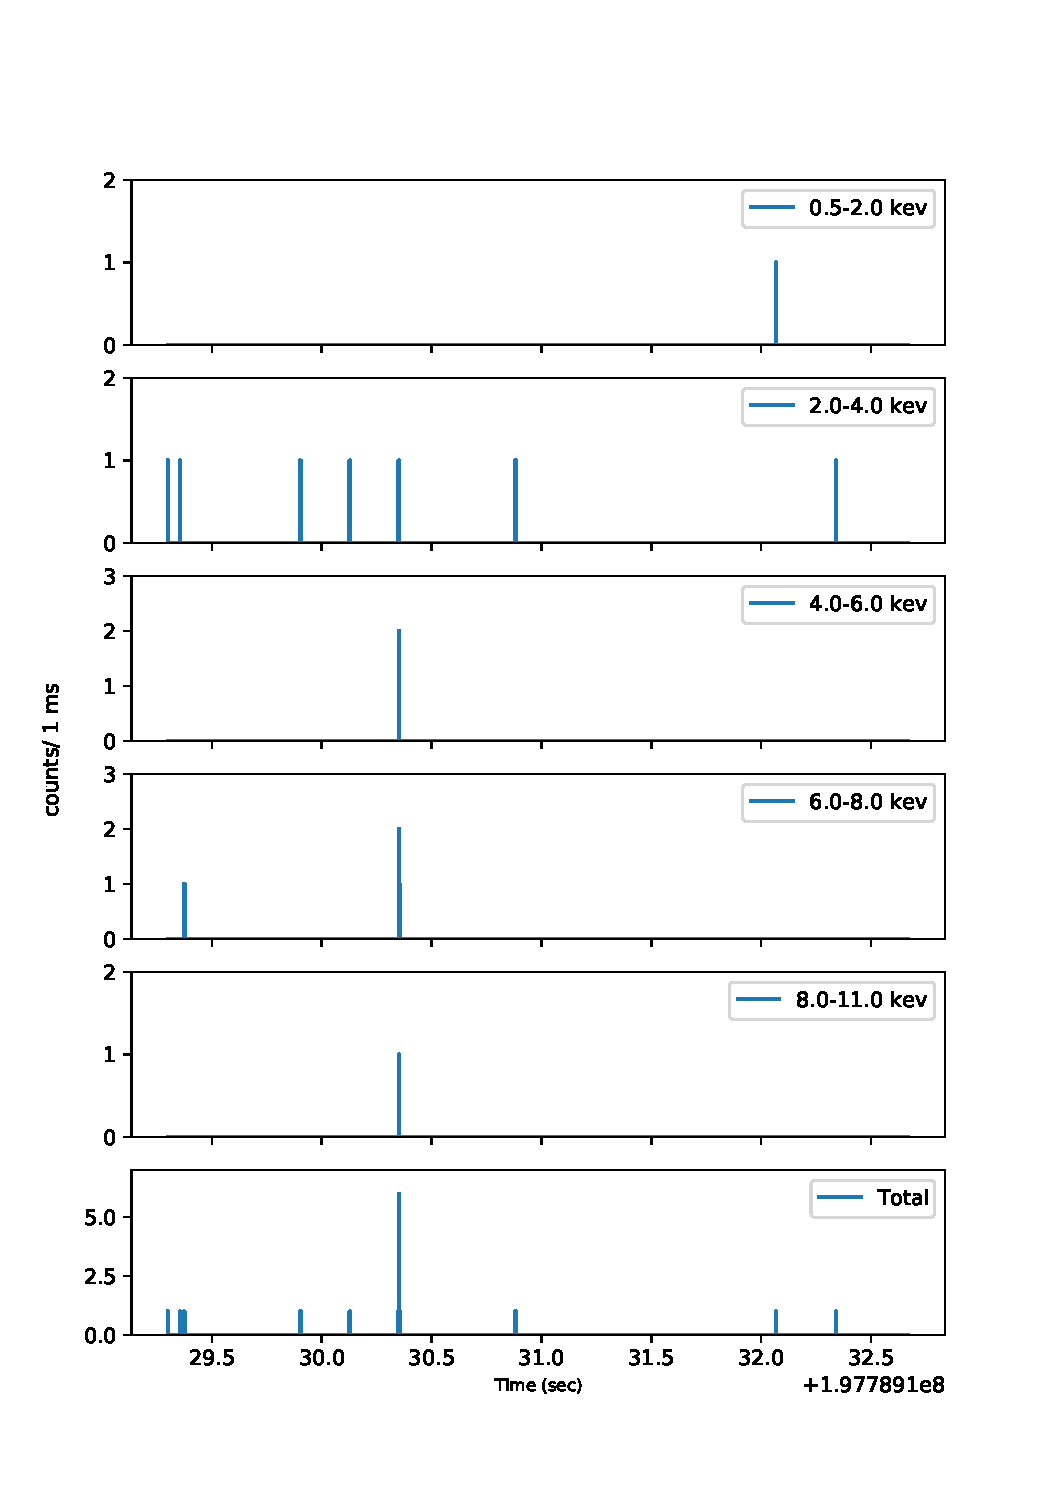
\includegraphics[trim=0cm 0cm 0cm 0cm, clip=false, scale=0.55, angle=0]{energy_plot_burst_801.pdf}
%	\caption{The 0.0015 s light curves of short X-ray burst in J1818$-$1607 in six energy bands. These energy bands lie in the range: $0.5-2$ keV, $2-4$ keV, $4-6$ keV, $6-8$ keV, $8-11$ keV. \abp{[Are we keeping this?]}}
%	\label{Figure:Figure1}
%\end{figure*}

\begin{figure*}[b]
	\centering
	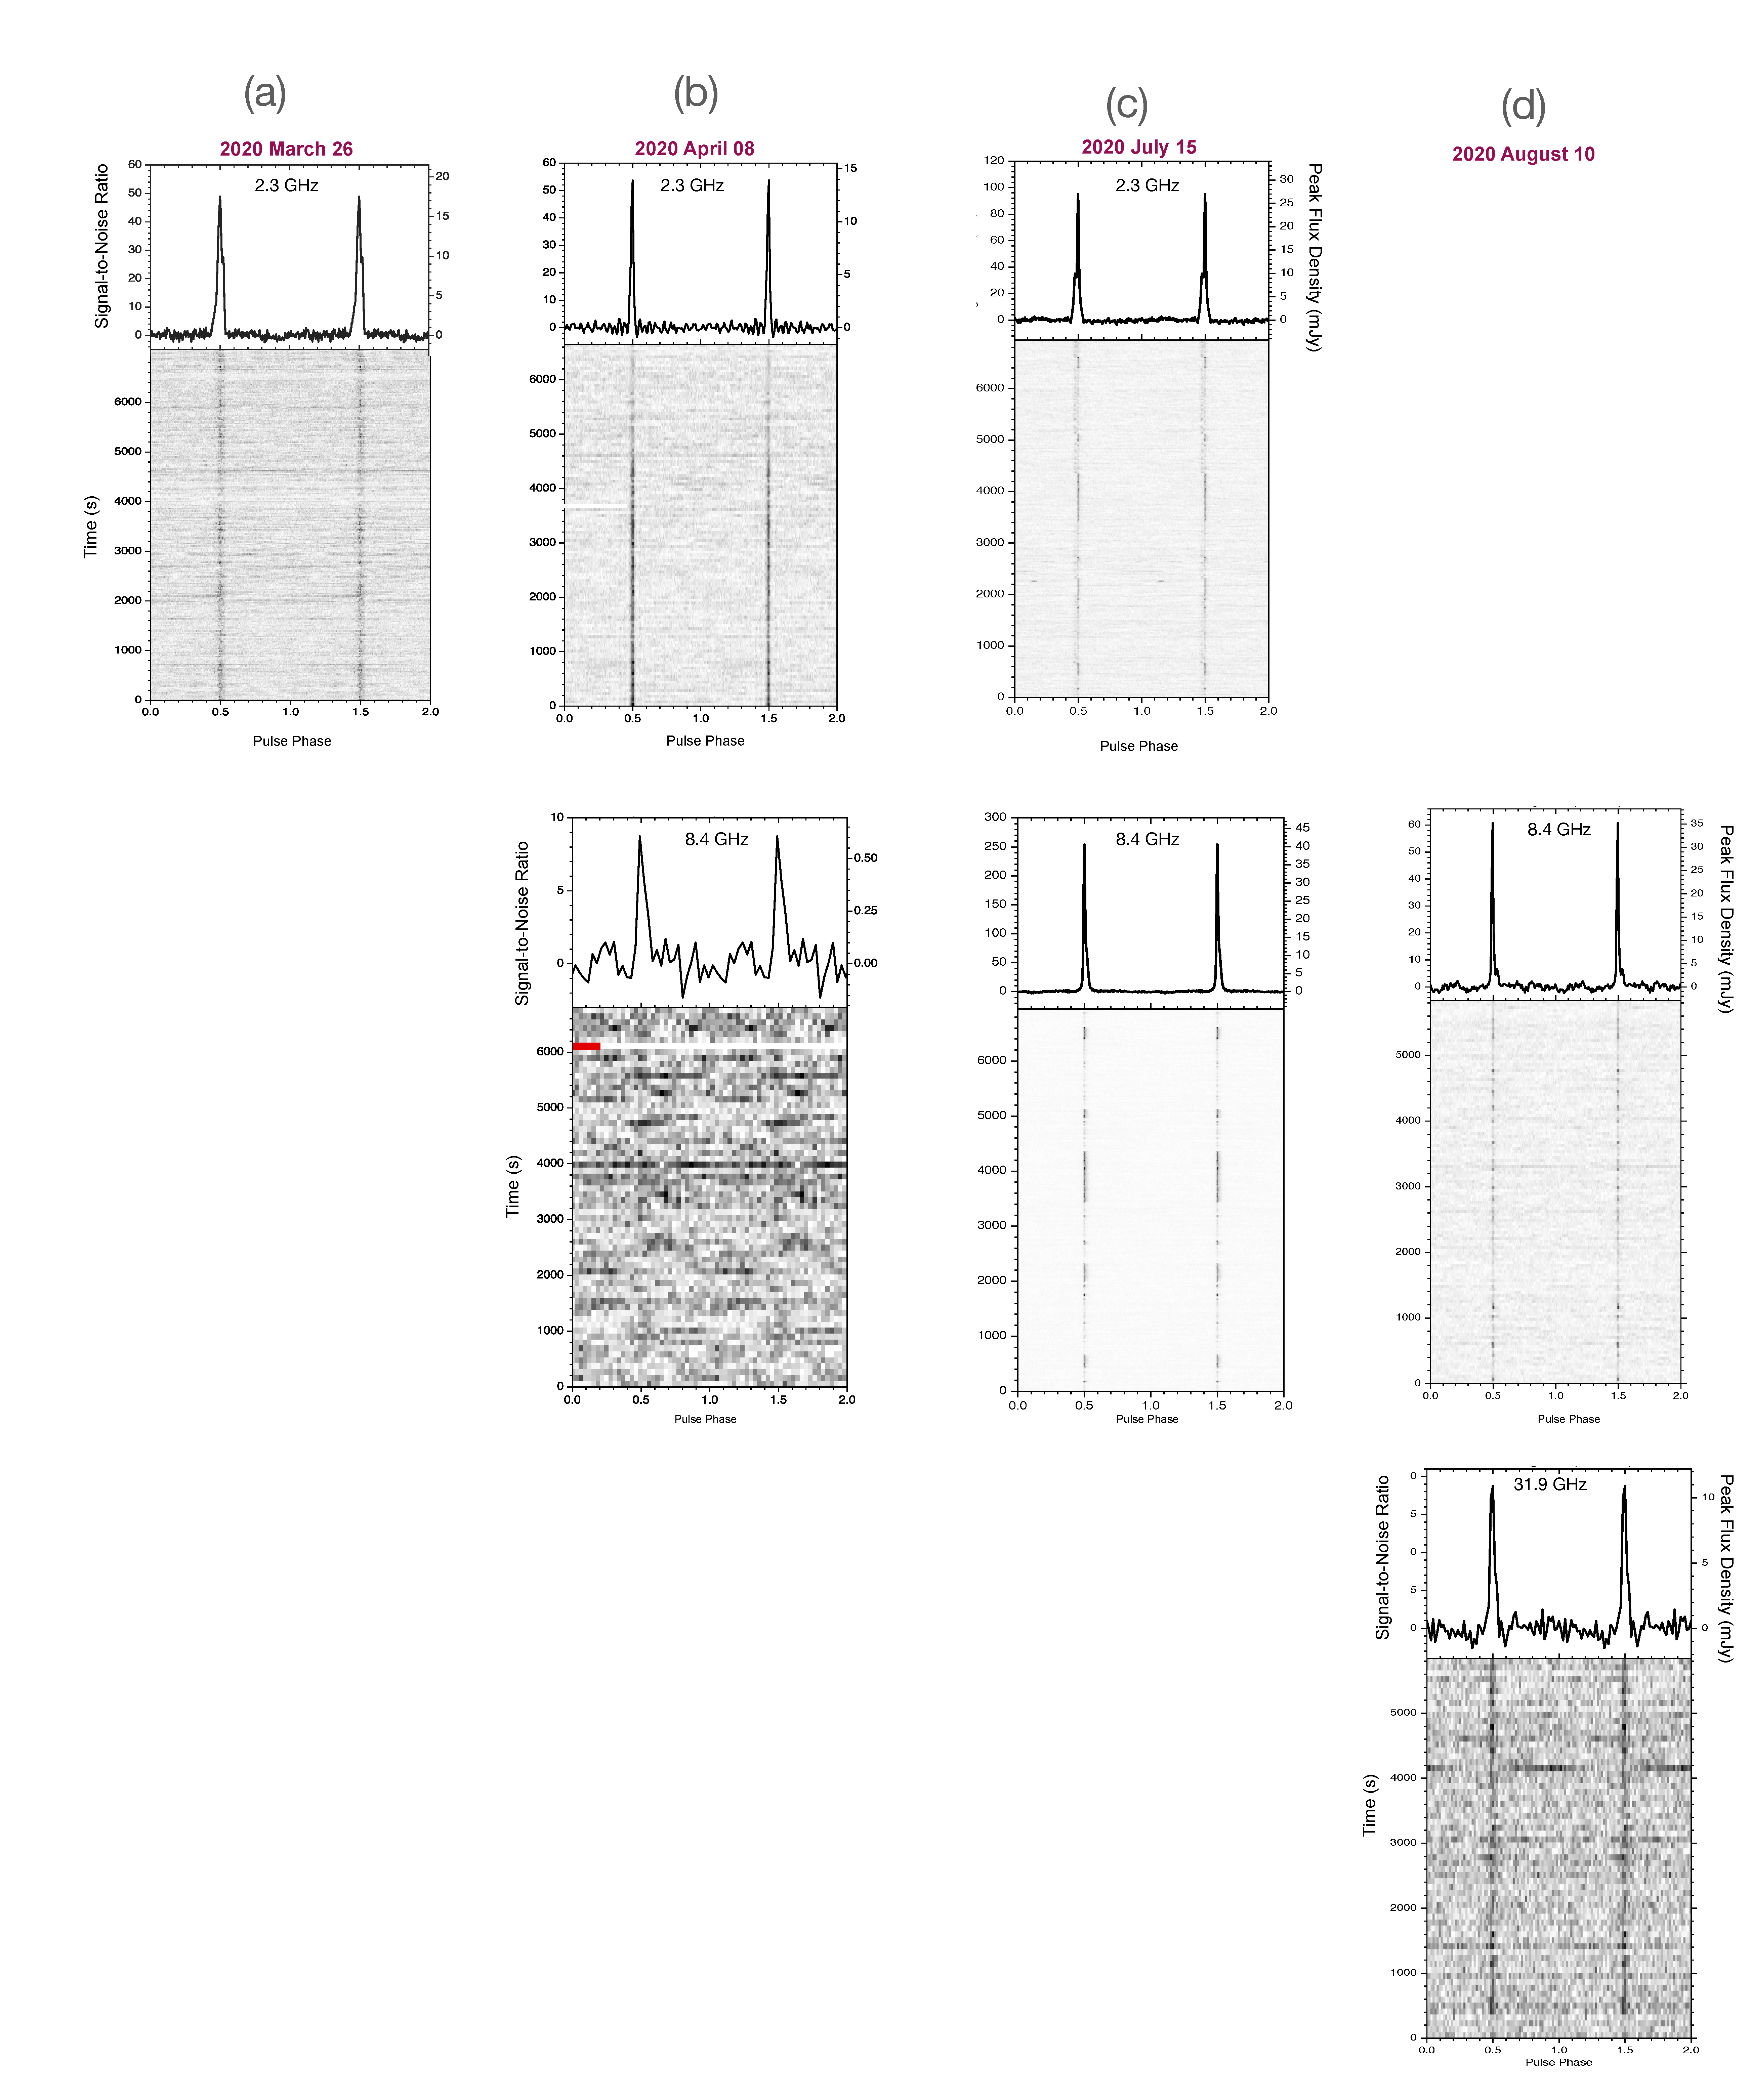
\includegraphics[trim=0cm 0cm 0cm 0cm, clip=false, scale=0.20, angle=0]{spectrum_radio_j1818.pdf}
	\caption{ Average pulse profile and time-resolved folded profile of Swift J1818.0-1607 at different epochs and frequencies (Table 1). Pulse profiles at (a) $S-$band for Epoch 3; (b) and (c) $S$ and $X$ bands for Epoch 4 and 5, respectively, and (d) $X$ and $Ka$ bands for Epoch 6. In (c), a variation in the flux density can be seen in both $S$ and $X$-band over the period of observation.}
	\label{Figure:Figure3}
\end{figure*}

\begin{deluxetable*}{llcccc}
    \tablenum{2}
    \tabletypesize{\small}
    \tablecolumns{6}
    \tablewidth{0pt}
	\footnotesize
	\tablecaption{Rotational Period and Flux Density Measurement of Swift J1818.0-1607}
    \tablehead{
        \colhead{Epoch} &
        \colhead{F0} &
        \colhead{$S$-band Flux Density} &
        \colhead{$X$-band Flux Density} &
        \colhead{$Ka$-band Flux Density} &
        \colhead{Spectral Index} \\
        \colhead{} &
        \colhead{(Hz)} &
	\colhead{(mJy)} &
        \colhead{(mJy)} &
         \colhead{(mJy)} &
	\colhead{}\\
        }
        \startdata
        	1 & .. & ...  & $<$ 0.05 & $<$ 0.08 & .. \\
	2 & .. & $<$ 0.05  &$<$ 0.03 & ... & .. \\
	3 & 0.7333684(2) & 0.80(2)  &$<$ 0.03& ... & $<$ -2.2 \\
	4 & 0.73335175(6) &  0.31(6) & 0.026(5) & ... & -1.9(2) \\
	5 & 0.7331469(2)  & 0.70(1) & 1.00(2) & ... & +0.3(2) \\
	6 & 0.73309715(8) & ... & 0.7(1) &  0.41(8) & -0.4(2) \\
        \enddata
        \tablecomments{Reported flux density Spectral index was obtained between two frequency bands during every epoch.\\}
        \label{Table:RadioResults}
\end{deluxetable*}
\subsection{Radio Profiles}

We searched all datasets for evidence of pulsed emission near the spin period of the pulsar after dedispersing the data. No pulsed emission was detected at Epoch 1 and Epoch 2 in both frequency bands. In Epoch 3, we detected a strong pulsed emission in the $S$-band after folding the data with a barycentric spin frequency of 0.7333684(2) Hz. It was derived from fitting a phase-coherent timing model (assuming a constant rotational frequency) to the pulse time of arrivals (ToAs) derived from sub-integrations across the observation duration. However, no pulsed emission was detected in $X$-band during this epoch. We plot the average pulse profile and time-resolved folded profile of J1818 in $S$ for Epoch 3 in Figure 1(a). 

Similarly, we have detected pulsed emission in both $S$ and $X$ bands with barycentric spin frequencies of 0.73335175(6) Hz and 0.7331469(2) Hz for Epoch 4 and 5, respectively. We plot the average integrated pulse profile and time-resolved folded profile in both frequency bands at these two epochs in Figures 1(b) and 1(c). A notable feature of the pulsed emission, during the July 15, 2020 observation (Epoch 5), is the large temporal fluctuation in J1818's flux density. In Epoch 6, the radio emission has been detected at both $X$ and $Ka$ bands with a measured rotational frequency of 0.73309715(8) Hz. We plot the average pulse profile and time-resolved folded profile in both frequency bands at this epoch in Figure 1(d). Spin frequencies from all epochs have been listed in Table 2 and plotted against their corresponding MJDs in Figure 2. We fit these points using a linear function to obtain $\dot{\nu} = -2.33(3) \times 10^{-11} $ s$^{-2}$, as an average estimate of $\dot{\nu}$ between March 26, 2020, and August 10, 2020.\\ 

In addition, we study the pulse morphology of J1818 across these observations. The $S-$band pulse profile shows a hint of a trailing second peak in the main component at Epoch 3, with no such indication at Epoch 4 and 5 (Figure 1b and c). Instead, the $S-$band pulse profile at Epoch 5 shows a leading secondary component. This agrees with the J1818 observation by \cite{marcus2020b}, reporting an emergence of a leading secondary component which causes an inverted spectrum in the 0.7 -- 4 GHz average pulse profile of J1818. Similarly, the $X-$ band profile has evolved from no hint of a second peak at Epochs 4 and 5 to a trailing second peak at Epoch 6. This aligns with the detection of the second peak in the main component in the 0.7 -- 4 GHz average pulse profile at later epochs (MJD 59074 -- 59109) in \cite{marcus2020b}. However, no second peak at the $X-$ band has been reported in a recent study of J1818 \citep{Huang2021}, likely due to the difference in the sensitivity of the telescopes. %We discuss these variations in pulse profiles in more detail in Section 4.1.
 
%In order to obtain accurate measurements, it requires timing analysis using phase-connected times of arrivals. \\ \abp{[I think we should remove these last two sentences and instead say that our measurement is consistent with Champion+2020, e.g. Fig. 9]} 

%\wam{I think we should also add a short subsection describing the pulse profile variability} \abp{[I agree.] - I have added a paragraph in the discussion section instead}

\begin{figure*}[b]
	\centering
	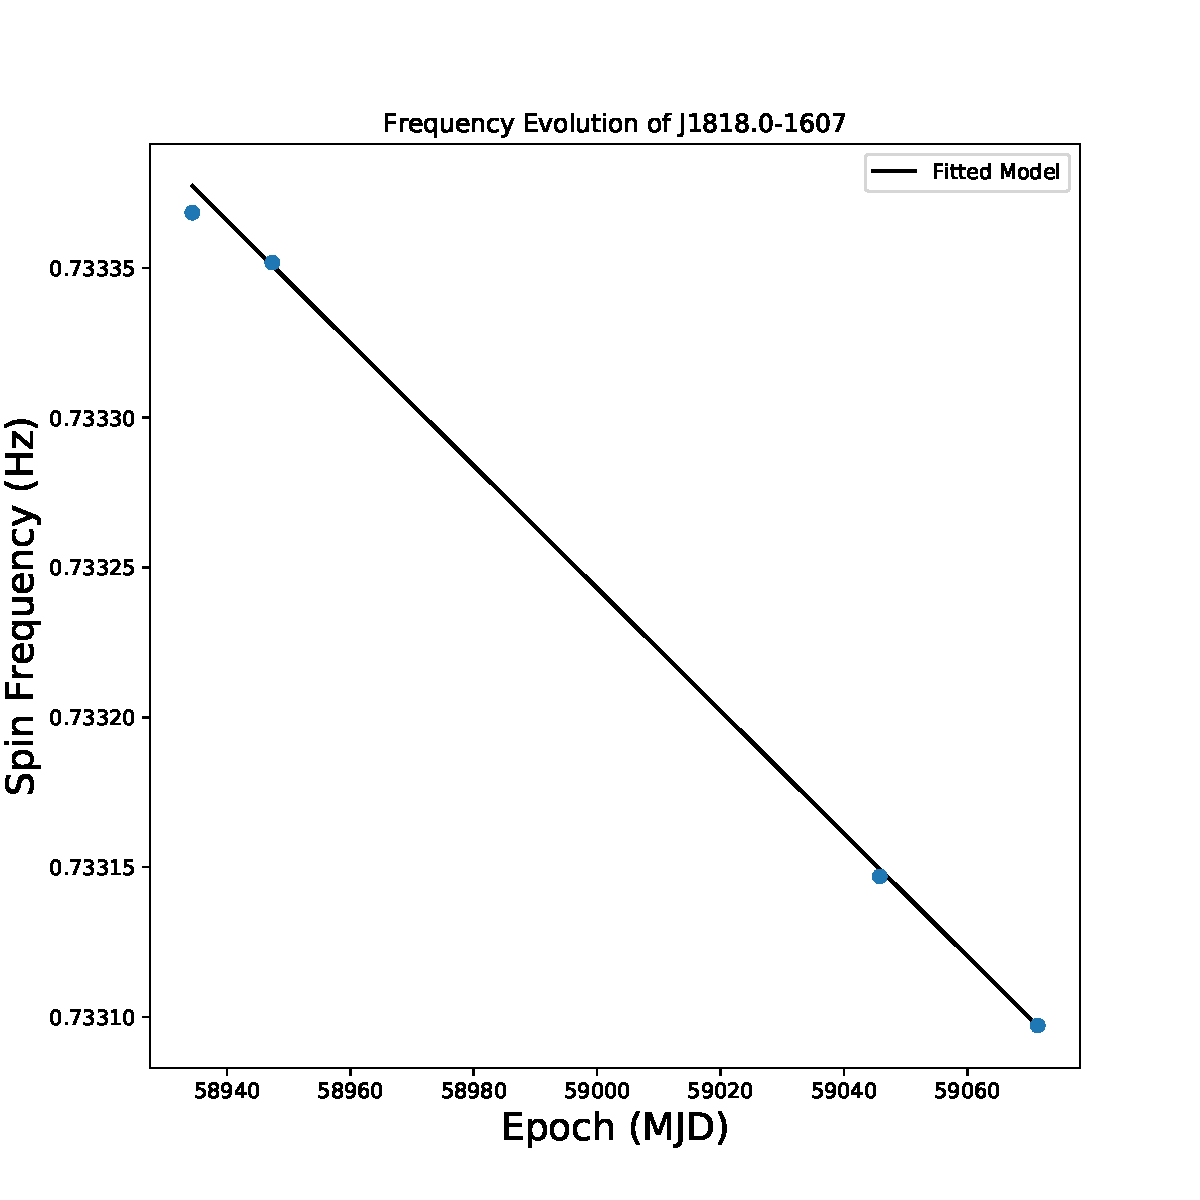
\includegraphics[trim=0cm 0cm 0cm 0cm, clip=false, scale=0.5, angle=0]{J1818-1607_frequency_evolution.pdf}
	\caption{ Change in spin frequency of J1818.0-1607 over four epochs. The error bars are smaller than size of the data points. We fit these point using a linear function to obtain average $\dot{\nu} = -2.33 \times 10^{-11} \pm 3.07 \times 10^{-13}$ Hz s$^{-1}$}%  \abp{[Explicitly state the results of the fit in the caption?]}
	\label{Figure:Figure2}
\end{figure*}


\subsection{Radio Flux Density and Spectral Index}

During Epoch 1, as there is no evidence of pulsed emission, assuming a 10\% duty cycle, we place a 7$\sigma$ upper limit on the flux density of $< 0.05$ and $< 0.08$ mJy at $X$ and $Ka$ bands using the radiometer equation. Similarly, for Epoch 2, the upper limits at $S$ and $X$ bands are $< 0.05$ and $< 0.03$ mJy. For Epoch 3, the mean flux density at $S$-band is 0.8(2) mJy, with an upper limit of $< 0.03$ mJy at $X$-band. Considering a power-law dependence of flux density with observing frequencies, we place an upper limit of $< -2.2$ on the spectral index. For Epoch 4, the mean flux densities at $S$-band and $X$-band are 0.31(6) mJy and 0.026(5) mJy, respectively. With a measured spectral index of $-1.9(2)$ between $S$-band and $X$-band, J1818 has a steep spectrum which is also evident in the pulse profile (Figure 1b). This is consistent with the average spectral index of $-1.8(2)$ associated with radio pulsars \citep{maron2000}. Similarly, for Epoch 5, the mean flux density at $S$-band and $X$-band are 0.7(1) mJy and 1.0(2) mJy, respectively, and a corresponding spectral index of +0.3(2). Between Epoch 4 and 5, the magnetars's flux densities have increased and the spectrum has inverted, which is quite typical of high magnetic field pulsars and radio magnetars. Moreover, the number of pulse components in the $S-$band changes between Epoch 4 and 5. For Epoch 6, the magnetar's mean flux density at $X$-band and $Ka$-band are 0.7(1) mJy and 0.41(8) mJy, respectively. Interestingly, the spectral index of J1818 between Epoch 5 and Epoch 6 evolves from +0.3(2) to -0.4(2), suggesting a spectral turnover at high frequencies. Since the flux density of J1818 at $X$-band is consistent between Epoch 5 and 6, this variation in the spectral index is unlikely due to time-dependent changes in the magnetar's flux. %Moreover, it appears that J1818's radio emission is evolving over time,
%The appearance of these different secondary components These variations in the flux density could be . Comment more about its similarity to other pulsars and magnetars?report a similar change in the spectral index in J1818 at lower frequencies. For three epochs, they find a double power law However, Seems like high frequency turnover has been seen in other magnetars such as SGR 1745-2900 and XTE 1810-197.  

%\abp{[We need to add a section in the discussion devoted to the spectral variability of this and other magnetars. We should mention the possibility of a spectral turnover, which is supported by the recent ATels from JBCA and Max Planck folks, but also possibly variability of the flux density that is both frequency- and time-dependent.] - done}

\begin{figure*}[b]
	\centering
	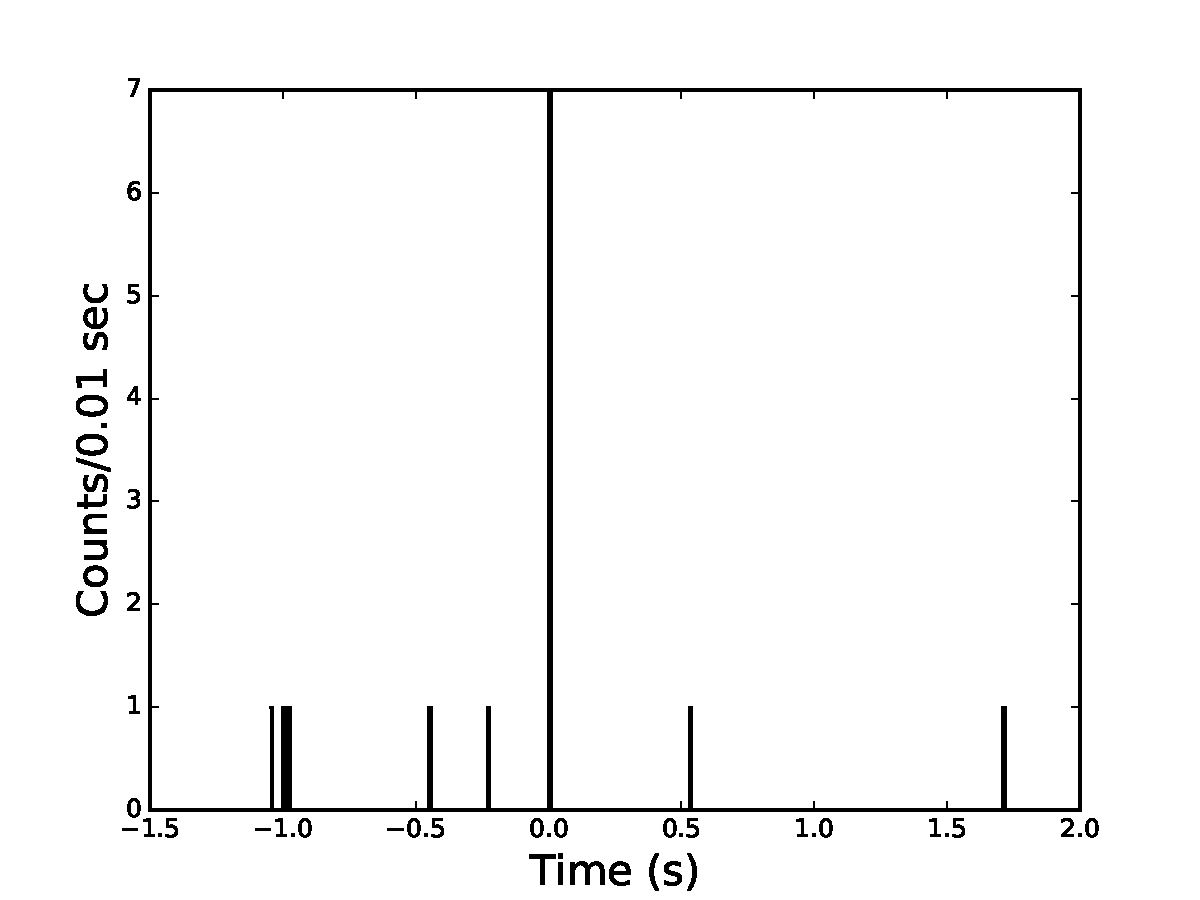
\includegraphics[trim=0cm 0cm 0cm 0cm, clip=false, scale=0.55, angle=0]{J1818_burst_light_curve.pdf}
	\caption{Light curve of a short X-ray burst in J1818.0$-$1607, in the energy range 0.3-10 keV (Section 3.3). The number of photons in this burst are 5 and its width is 0.0015 s. It was observed using the NICER telescope with observation Id:3556011801.} 
	\label{Figure:Figure3}
\end{figure*}

\subsection{X-ray Bursts}

We carried out a search for X-ray bursts in both X-ray observations (see Section 2.2) using unbinned event times. We employ the technique of Bayesian blocks \citep{scargle12} which obtains optimal bins for a given dataset. This is a robust technique as it does not depend on the sampling or bin size of a dataset and can detect local structures in highly variable datasets. The datasets are first divided into optimum segments (blocks) such that there is no overlap between them and all model parameters, such as event rate, are constant within each block. The boundaries where a statistical model undergoes an abrupt change are called edges. These edges are used to form optimal histograms which help in identifying local structures \citep{lin13}. This prior distribution of blocks ($ncp_{prior}$) is obtained using Equation 21 in \cite{scargle12}, which depends on the number of events ($N$) and the false probability ($p0$). In this paper, we use an inbuilt Bayesian  Block function from AstroPy, with $p0 = 0.05$.


In our first X-ray observation of J1818, the edges overlap with the good time intervals (GTIs) suggesting that there are no bursts during this observation. However, for the second X-ray observation, we note that the number of edges is more than the number GTIs. Upon a closer investigation, we find a block at MJD 58947.2201 with a sudden increase in the count rate in a short duration, suggesting a soft x-ray burst. The number of photons in this burst is 5 and its duration is 0.0013 s. Its width has been obtained from the size of the representative Bayesian block. The mean count rate for this observation is 1.2 counts s$^{-1}$, which has been obtained from the spectral fitting in the energy range of 0.3--10 keV \citep{hu2020}. For the duration of this burst, the mean count is 0.002. Assuming a Poisson distribution, we obtain the false alarm probability of this burst to be 2.7e-16. We have plotted the light curve of this burst in Figure 3. However, due to the low number of counts in this burst, we were unable to fit its spectrum.

%  We estimate the signal-to-noise ratio (SNR) ($N/\sqrt(N+B)$) of this burst to be 2.5 $\sigma$ using the estimated background rate (b). From these SNRs, we conclude that this burst is statistically insignificant.%We find the total significance of this burst to be $2.5\sigma$, % <<THE ESTIMATE OF SIGNIFICANCE FOR INDIVIDUAL SPECTRA IS EVEN LOWER SO I WONDER IF WE SHOULD INCLUDE THAT>> %\textit{nicer\_bkg\_estimator}\footnote{\url{https://heasarc.gsfc.nasa.gov/docs/nicer/tools/nicer_bkg_e st_tools.html}}. It is a space weather based method (Gendreau et al., in prep) which obtains the background spectra of an observation based on the time-dependent particle background, optical loading from the Sun, and the diffuse sky background. 

 
%%  Obtain the significance of burst in each energy range
%The top panel shows burst in the .. ..  We obtain various light curves with binsizes ranging from 0.001 till 1 seconds (Figure ). At both epochs we obtain one bursts which persists across these binsizes. 

%\begin{figure*}[b]
%	\centering
%	\includegraphics[trim=0cm 0cm 0cm 0cm, clip=false, scale=0.25, angle=0]{J1818_observation_overlap.pdf}
%	\caption{Overlapping observations in X-ray and Radio at both epochs.}
%	\label{Figure:Figure2}
%\end{figure*}

\subsection{X-ray Profiles}
 
We obtain absolute X-ray phases for both epochs using PINT built-in functions \citep{Luo2019}, and the ephemeris obtained from contemporaneous radio analysis. We fold the X-ray data and obtain average X-ray profiles, one for each epoch. This is done using NICERSoft program \footnote{https://github.com/paulray/NICERsoft}, which uses the absolute phases, and filters out events with energies less than 2 keV and greater than 6 keV to select the most sensitive band of NICER telescope. In Figure 4, we plot the average X-ray pulse profiles (black) as well as the phaseogram for both epochs. Note that for Epoch 4 (Figure 4b), GTIs before and including the tentative X-ray burst have been excluded. The pulsed X-ray emission is consistent within the observation duration for each epoch, with no indication of any glitch. The RMS pulsed fraction \citep{an2015} for Epoch 3 and Epoch 4 are $0.31 \pm 0.02$ and $0.36 \pm 0.03$, respectively. This increase in the pulsed fraction is consistent with those reported in \cite{hu2020}. We note that the X-ray pulse profile in the second observation has more structure as compared to that of the first one.
%(MAYBE COMPARE THE FITTING PARAMETERS).

To investigate if there is any phase correlation between our simultaneous observations in radio and X-ray, we overlay the $S$-band average profiles (red) on X-ray profiles for both epochs. The location of the pulse peak in the X-ray profiles was obtained by fitting a sinusoidal function (blue). At both epochs, the peak of the radio pulse profile at $S$-band leads the X-ray pulse profile with a phase offset (in phase cycles) of $0.40 \pm 0.03 $ and $0.33 \pm 0.03$, respectively. This offset implies that the peaks of radio and X-ray are almost misaligned with the radio occurring at X-ray pulse minimum. We validated this procedure by comparing the radio and X-ray profiles of the Crab pulsar. We confirmed that the peak of its radio profile at the S-band aligns with the peak of its X-ray profile, as expected \citep{hankins2007}. We analyzed the recent NICER observation of J1818 in February 2021, to further test this phase misalignment, but no pulsed emission was detected in the X-ray.
 %following the same technique, we also measure the phase offset between X-ray and radio profiles of Crab pulsar to verify our strategy.}%This phase offset has been seen in case ofother magnetars such as XTE J1810-197 \citep{pearlman2020bright}.  Mapping these phase differences to emission height can result in difference of about ( radius of light cylinder =  cP/2pi = 65158 km )  <<EMISSION HEIGHT>> %It is likely due to offset in the emission region?

%. Averaged X-ray pulse profiles (blue), with a binsize of 0.5 second, have been plotted in Figure 3. The frequency of this magnetar changes from $7.3337E-01 \pm 1.036 E-07$  to $7.3335E-01 \pm 9.550E-08$ between two epochs. Since this is a very young magnetar,

%\abp{[I would have said that the X-ray profile peak lags the radio profile peak, but I don't think we should mention this until we do an experiment with a slow X-ray/radio PSR with the DSN/NICER in Madrid to confirm the timing accuracy. If we're short on time, we can add this during the review stage. For right now, let's just measure the relative offset during the two epochs, and comment on whether it variable in time.]}

\begin{figure*}[b]
	\centering
	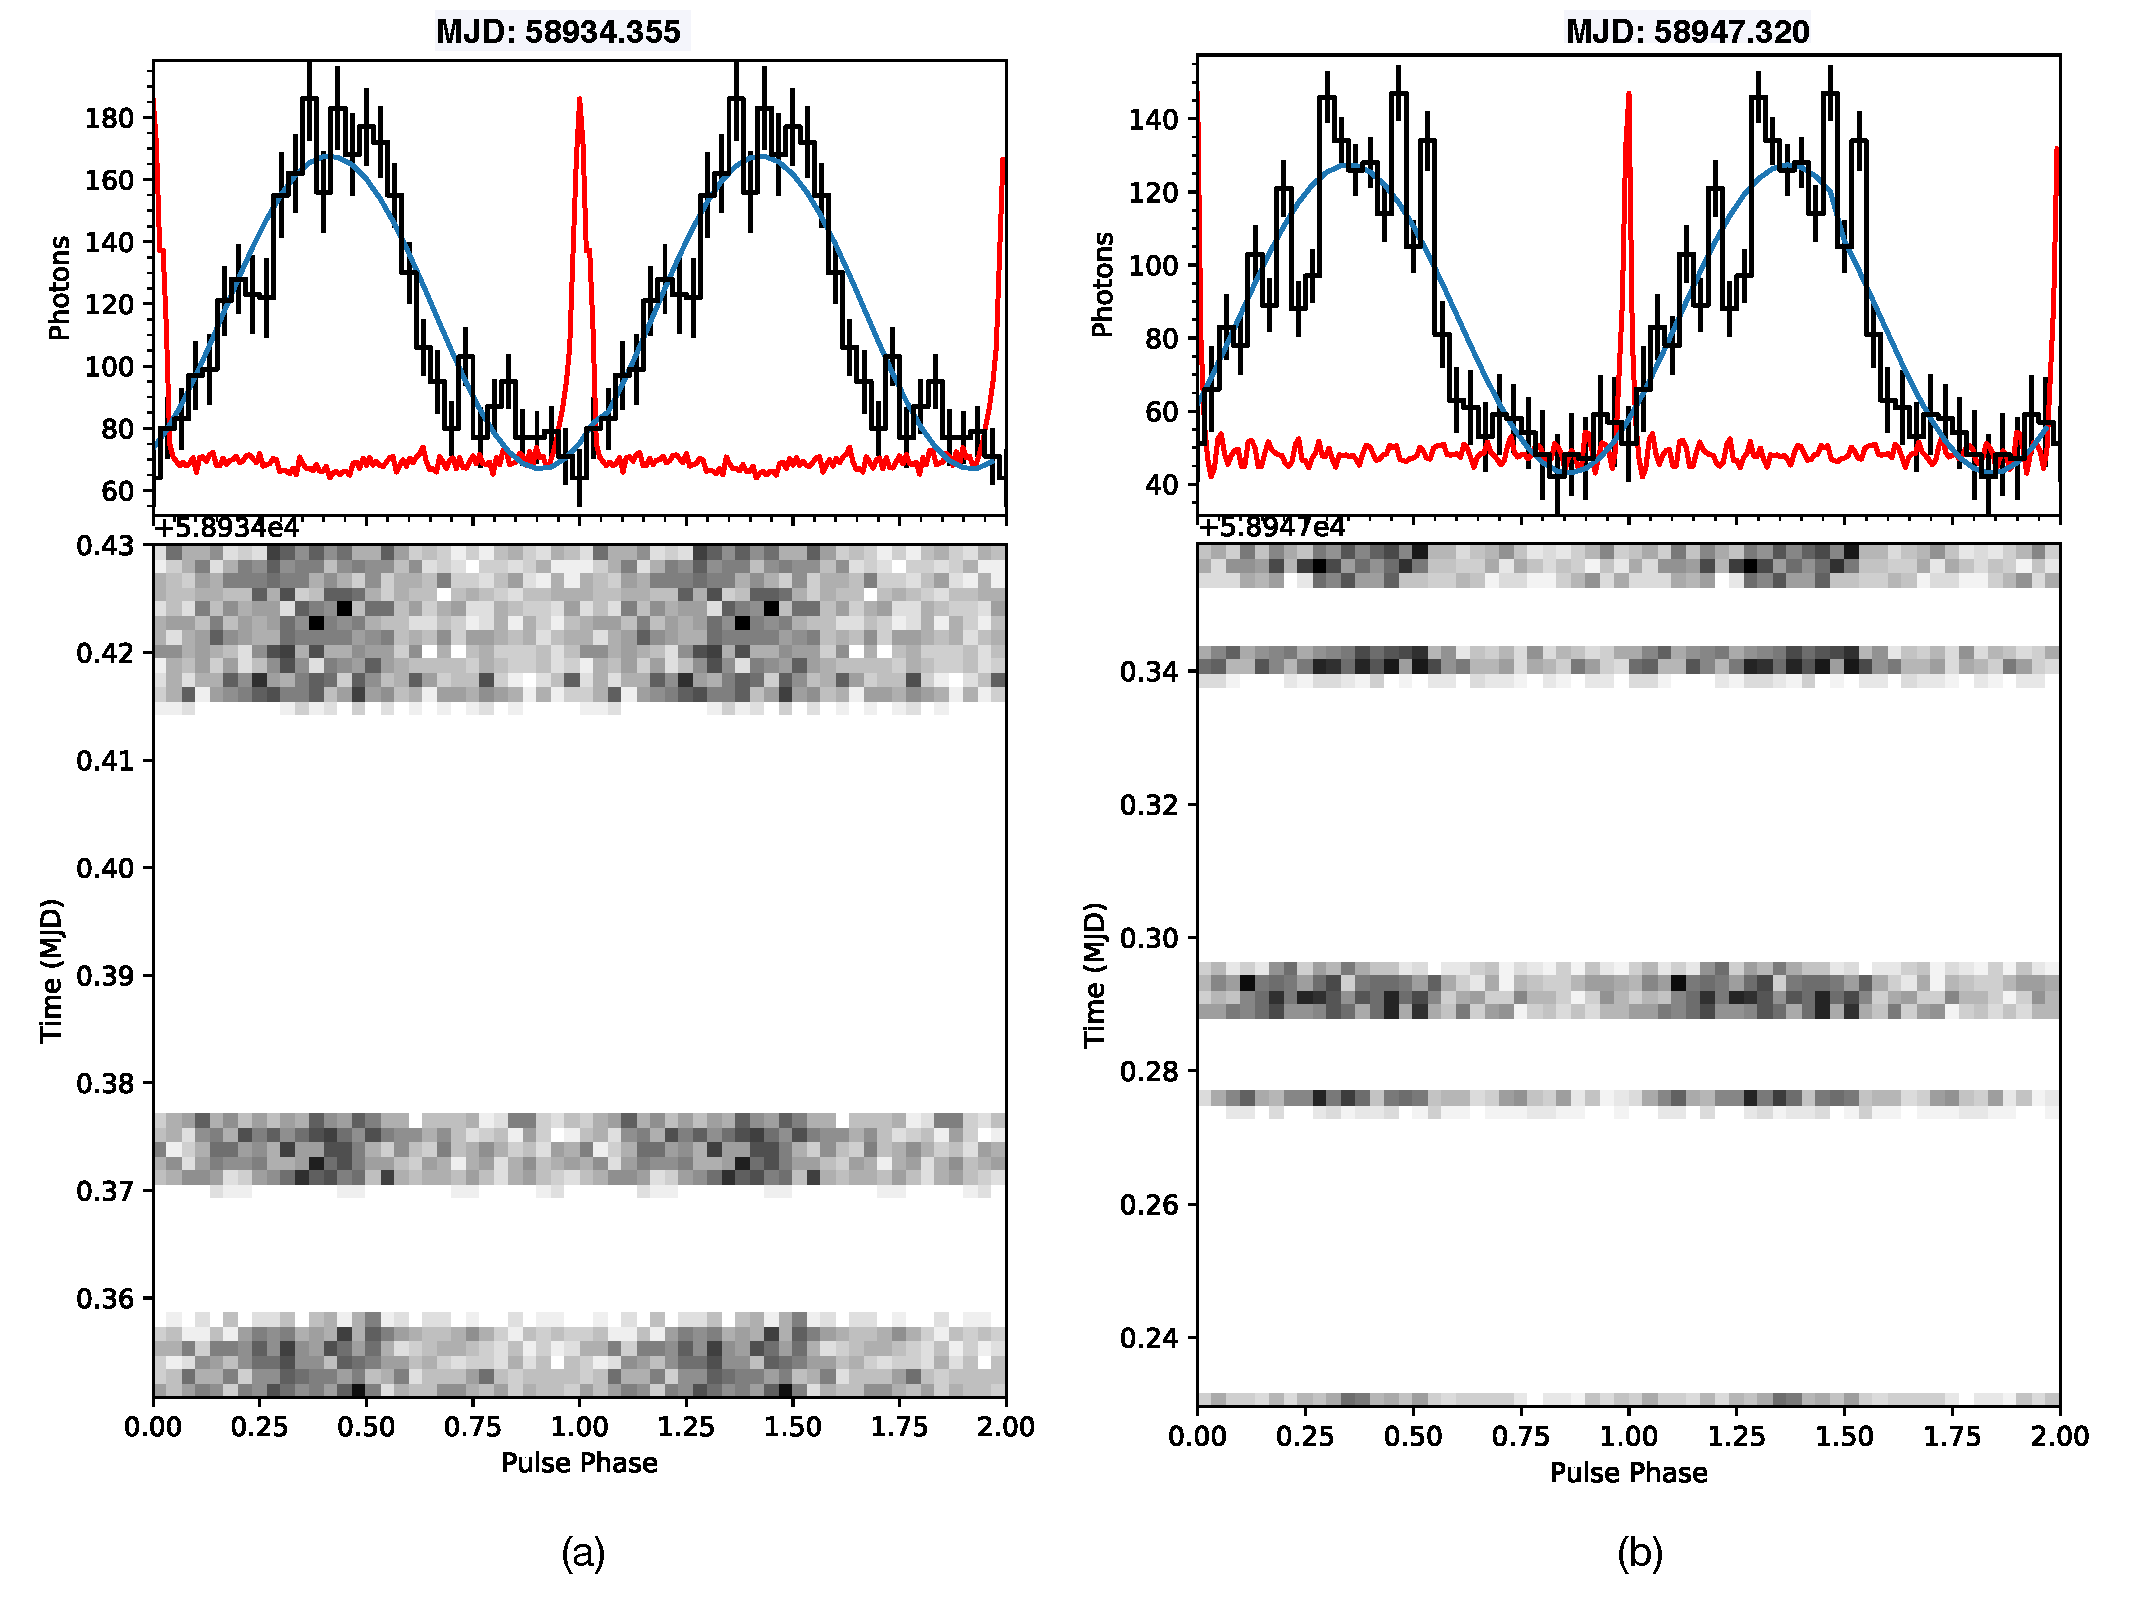
\includegraphics[trim=0cm 0cm 0cm 0cm, clip=false, scale=0.4, angle=0]{average_phaseogram.pdf}
	\caption{ Integrated pulse profiles and phaseogram of J1818-1607 at X-ray (black) during MJD 58934.35 (panel 1) and 58947.33 (panel 2). We fit each X-ray profile using a sinusoidal function (blue) and overlay the corresponding average pulse profile at $S$-band (red). The phase offset between radio and X-ray profile are $0.40 \pm 0.03 $ (a) and $0.33 \pm 0.03$ (b).}%\abp{Remove white space at the start, in the bottom panels. Also, don't use scientific notation for the MJD times along the y-axis, and use fewer bins in the X-ray pulse profile.]} 
\end{figure*}

\section{Discussion}

\subsection{Comparison with Magnetars}

%We compare our observations of J1818 with those of other magnetars. Most of the magnetars have been found to be in the plane of the Galaxy, suggesting the young age of these sources \citep{Tendulkar 2013}. where is this source in the Galaxy-- how does it compare to other magnetars?%Similar to other radio magnetars J1818 also exhibits periodic radio emission with a spin period same as the persistent X-ray emission. %Contrary to XTE J1810-197, which shows quiescent, no such feature has been yet detected since its discovery in March 2020.


%We compare our observations of J1818 with those of other magnetars. 
We search for X-ray bursts in our NICER observations of J1818 and detect one X-ray burst. In a recent study, \cite{hu2020} reported additional 18 X-ray bursts from this source, detected using the NICER telescope. We also report the averaged X-ray pulsed emission from J1818 from two epochs in Figure 4. Thus, J1818 shows both persistent X-ray emission as well as a prolific number of X-ray bursts, a hallmark of magnetars.

Using the above estimated $\dot{\nu}$ value (see Section 3.1), we obtain an average period derivative, $\dot{P}$ of $4.34 \times 10^{-11}$ s s$^{-1}$ (Figure 2). We estimate the dipolar B-field strength at the equator ($\propto \sqrt(P \dot{P})$) to be $2.5 \times 10^{14}$ Gauss and the characteristic age ($\frac{P}{2\dot{P}}$) is about 500 years. These overall characteristics compare well with other magnetars. Our measurement of $\dot{P}$ as compared to recent studies \citep{esposito20, lower2020} is about two times smaller, and matches with those by \cite{Champion_2020, hu2020}, and \cite{Huang2021}. Note that all the estimates of $\dot{F}$ are unreliable due to the strong timing noise in this source; thus, the true age significantly differs from the spin-down age. This is not surprising as $\dot{F}$ is often observed to vary in magnetars, especially during periods of bursting activity. Moreover, the estimated characteristic age is not a good indicator of its age as it assumes magnetic dipole radiation, which is likely not the case for magnetars. Perhaps an estimate of proper motion will provide a more robust estimate of age if an association with a supernova remnant is found \citep{blumer2020,lower2020, Gaensler2000}. Moreover, kinetically derived age is independent of an emission mechanism.  

%, however, our observations are based on a longer observing span.
From our radio analysis, we see a large variation in the flux density of J1818 over various timescales, ranging from hours to months (Figure~1). At $X$-band, it goes from a null detection at the first few epochs to a $5\sigma$ detection from Epoch 4 onward. The flux density of J1818 at $X$-band increases by a factor of 40 between Epochs 4 and 5. Similarly, there is a null detection at $Ka$-band in Epoch 1, with a flux density of 0.41 mJy in Epoch 6. Moreover, during Epoch 5, there is a change in the flux density on the timescale of hours during our observation at both $S$ and $X$-band (Figure 1c). In contrast to our null detection in the first few epochs, \cite{Champion_2020} detect pulse emission in Epoch 1 at 1.5 and 2.5 GHz, and Epoch 2 at 1.5 GHz. As the observing frequencies in \cite{Champion_2020} are lower than our corresponding frequencies (Table 1), our non-detections are due to the steep spectrum of J1818 at these epochs. Similarly, there is a change in the spectral index of J1818 between $S$-band and $X$-band as it goes from a steep spectrum of $< -2.2$ at Epoch 3 to a flat spectrum of $+0.3$ at Epoch 5, over a period of about three months.  A similar variation in the spectral index ($-0.97$) has been reported in a recent observation of J1818 \citep{Liu2020}. In Epoch 6, we see a spectral turnover with an index of $-0.4$ between 8.4 GHz and 32 GHz, consistent with a recent estimate of $-1.4$ between 86 and 154 GHz \citep{Torne2020}. 


The above characteristics of J1818 are analogous to other radio magnetars \citep{lazaridis2008, torne2015}. These variations could be intrinsic in origin, and maybe a result of frequency-dependent variability of the magnetar's intensity on short timescales, or due to the untwisting of magnetic field lines, which could also affect the pulse profile \citep{scholz17}. J1818 also shows a significant change in its pulse morphology at both $S$ and $X$ bands over the span of our observations, similar to other radio magnetars such as XTE 1810-197 and SGR 1745-2900 \citep{camilo2007, pearlman2018}. In addition, we also see a variation in the X-ray pulse profile as it becomes slightly more complex in Epoch 4 as compared to Epoch 3 (Figure 4). The flattening and high-frequency spectral turnover of J1818 spectra are accompanied by the emergence of secondary components as has been pointed out by \cite{marcus2020b} and can also be seen in our observations at Epoch 5 and 6. These time-dependent variations in the flux density can also be caused by extrinsic effects, such as scintillation. Using the galactic electron density model, NE2001 \citep{cordes2002}, we estimate the scintillation time and bandwidth at $S$-band to be $\sim 2$ s and 117 Hz, and $\sim 11$ s and $\sim 35$ kHz at $X$-band. These estimates are also consistent with the YMW16 model \citep{Yao_2017}. Based on these estimates, the scintles at both bands get averaged out in frequency but not necessarily in time. Hence, scintillation is one of the possible contributing factors to the observed temporal variations. Unfortunately, more simultaneous observations are required to further explore this connection between the changes in pulse profiles at both radio and X-ray with those in the spectral index. However, we note that J1818 shows the largest variation in the spectral index over a span of six months. 


%These variations in J1818 put it in the same category as other magnetars and suggests its young age as the underlying reason. They also report two emission modes possibly contributing to this changes. They note that this change in the spectral index has stopped in the later epochs suggesting that the process has calmed down. However, due to the lack of high cadence an association with the high energy burst activity and radio emission are difficult to make.  
% scintillation time estimates are As our frequency resolution is lower than tese estimates, we can not resolve this variation in frequency,


\subsection{Comparison with Radio Pulsars}

The spectral index of J1818 shows a transition from steep to flat spectrum, unlike typical radio pulsars which have a stable steep spectral index of $-1.8 \pm 1$ \citep{maron2000}. In this aspect, it is similar to the transitional magnetar, PSR J1119-6127, which has also been found to emit X-ray bursts \citep{Gogus__2016}. However, similar to typical radio pulsars, both the spin period (0.33 s) and magnetic field ($4.3 \times 10^{13}$ Gauss) of PSR J1119-6127 are small as compared to J1818. 
The distinction between radio pulsars and magnetars arises due to the difference in their measured X-ray luminosities likely caused by a difference in underlying emission mechanisms. In radio pulsars, magnetic dipole radiation is the dominating emission process \citep{kramer09}; however, in the case of magnetars, it is the decay of its strong internal magnetic field \citep{kaspi2017}. So far, about 90 radio pulsars have been found to have X-ray emission \citep{becker2009}. Their properties vary depending on their characteristic age. Young pulsars, such as the Crab pulsar, are believed to emit non-thermal X-ray emission due to magnetospheric emission from charged particles, and their pulse profiles from both X-ray and radio align in phase \citep{becker2009}. Middle-aged pulsars, such as Vela, have been found to show thermal X-ray emission due to thermal cooling and heated polar caps. A few old non-recycled pulsars have been found to show both radio and X-ray emission, likely non-thermal, as their surface is not hot enough to produce thermal emission. For example, B1929+10 and B0950+08 are old pulsars, which exhibit both X-ray and radio emission, but their pulse profiles are anti-aligned \citep{Becker_2006}. However, the exact reason for their misalignment is still unknown. %In case of aged pulsar such as Vela neutron cooling causes the thermal emission. The temperature of neutron star surface diminishes with age. Millisecond pulsars ...


In the case of J1818, we find that radio and X-ray pulse profiles are misaligned (see Figure 4) with a phase offset of $0.40(3)$ at Epoch 3 and $0.33(3)$ at Epoch 4 in phase cycles. A similar phase offset has been seen in another magnetar, such as XTE J1810-197, of about $0.11 \pm 0.05$ between the X-ray and radio observations \citep{pearlman2020bright}. One possible way to obtain such phase offsets is due to thermal emission at X-ray and non-thermal emission at radio. A recent study \citep{hu2020} suggests that the X-ray emission in J1818 is likely thermal, as its spectrum is fit using a blackbody. This aligns with the theoretical prediction of the X-ray emission originating from the hotspots in the magnetars, which form as a result of charges in the open field lines (j-bundles) hitting the surface of the magnetar \citep{beloborodov2009}. The observed phase offset can be explained by the radio emission being caused by the closed magnetic field lines rather than the open j-bundles, which are much thicker. As J1818 is a relatively young source as compared to XTE J1810-197, it is likely to have a more twisted magnetosphere. This causes an inflated poloidal magnetic field, which shrinks as the magnetosphere untwists and the size of the hotspot reduces. This explains the observed increment in the pulsed fraction of J1818 over two epochs, suggesting a shrinkage in the size of polar hotspot \citep{hu2020}.  %which can further contribute to the change in the location of the centroid, hence, the marginal change in the phase offset. As a magnetar evolves over time, the flaring would reducing, which 

Another possible explanation is the difference in the relative emission heights of X-ray and radio emission, which can also explain the change in linear position angle over time as noted by \cite{marcus2020b}. However, a phase offset of $\sim0.4$ (phase cycles) in J1818 corresponds to the difference in emission heights of about $1.6 \times 10^5$ km which is about three times larger than its light-cylinder radius ($6.5 \times 10^{4}$ km). This likely indicates that radio emission is likely not originating above the hotspot of the magnetar's surface. Moreover, the large polarization angle swing in J1818 was observed at only one epoch \citep{marcus2020b}, which is not simultaneous with our observations, making it more difficult to draw any strong connection between them. Observations at both radio and X-ray, with simultaneous measurements of polarization angle, will enable us to determine the exact location of these emission regions in magnetars.
    
 %(change in the location of centroid) %Similarly, J1119-6127 despite being a young pulsar  ($\sim 1000$ yr) has been found to show thermal X-ray emission \citep{}, which align with radio profile. - actually not true - no such evidence have been found.
%Due to its magnetar like properties such as X-ray bursts, transitional magnetar PSR J1119-6127 \citep{Gogus__2016}, serves as a bridge between radio pulsars and magnetars. Similar to J1818, J1119-1627 shows steep spectra with a large variation in spectral index unlike typical radio pulsars which have a stable steep spectral index of $-1.8 \pm 1$ \citep{maron2000}. %This on comparing with transitional pulsar such as J1119- on a higher side. However, the average $\dot{P}$ value is larger than radio pulsars.  


%compared to crab pulsar, pulsed fraction of vela is very small (7\%) - it shows thermal contribution - They are young enough to have high surface temperature to have detectable thermal emission and undergo cooling over time%X-ray bursts have been detected from hese sources have spin period of 0.33 and 0.41 s with magnetic field strength of the sources is ... and ... , respectively. Both magnetic field and \abp{[This part of the paper would strongly benefit from a discussion of the spin-down vs. X-ray luminosity of magnetars, etc...]}Similar to the Crab pulsar \citep{}, J1818 shows pulsed X-ray emission. In addition, there is an phase offset of <0.13 sec between the radio and X-ray observations. \abp[{See above comment about mentioning phase offset between radio/X-ray profiles.]} An offset of has been found in case of crab pulsar as well. I think this can be explained due to the difference in the emission heights at these two frequency bands. 


%Future study of phase-connected timing estimates will help better constrain the evolution of J1818. 

\section{Conclusion}
We study J1818 at multiple radio frequencies including the 32 GHz, over a span of about six months. We see a variation in its pulsed emission and flux density on the timescales of a few minutes to months. In addition, we note that J1818 shows a spectral turnover at higher frequencies, and has the largest change in the spectral index among other radio magnetars over a span of six months. These characteristics solidify its placement amongst the most intriguing radio-emitting magnetars, and an average estimated characteristic age of $\sim 500$ yrs further helps us in bridging the gap between magnetars and pulsars. Using our simultaneous X-ray and radio observations, we measure a large phase offset between their pulse profiles, which we attribute to the X-ray emission originating from the open field lines as opposed to the radio originating from the closed field lines. Future observations of this source will help us determine its true characteristic age, and measure how the phase offset between X-ray and radio pulse profiles evolves over time. %can help us govern the evolution of its magnetosphere.
 
 \section{Acknowledgments}

A.B.P. acknowledges support by the Department of Defense~(DoD) through the National Defense Science and Engineering Graduate~(NDSEG) Fellowship Program and by the National Science Foundation~(NSF) Graduate Research Fellowship under Grant~No.~\text{DGE-1144469}.

We thank the Jet Propulsion Laboratory's Spontaneous Concept Research and Technology Development program for supporting this work. We also thank Dr.~Stephen Lichten for providing programmatic support. In addition, we are grateful to the DSN scheduling team (Hernan~Diaz, George~Martinez, and Carleen~Ward) and the CDSCC and MDSCC operations staff for scheduling and carrying out these observations.

A portion of this research was performed at the Jet Propulsion Laboratory, California Institute of Technology and the Caltech campus, under a Research and Technology Development Grant through a contract with the National Aeronautics and Space Administration. U.S. government sponsorship is acknowledged.

\bibliographystyle{yahapj}
\bibliography{references} 
\end{document}
